
\begin{question}
Solve the system of equations.

\[\begin{aligned}
5 x^{2} - 10 x + y &= -88 \\
5 x + y &= -28
\end{aligned}\]
\end{question}

\begin{solution}
There are two solutions.

\[(-3,-13) \text{ and } (-4,-8) \]

This system represents a parabola and a line.

\begin{figure}
\centering
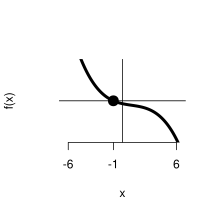
\includegraphics{unnamed-chunk-2-1.pdf}
\caption{plot of chunk unnamed-chunk-2}
\end{figure}
\end{solution}

